\chapter{Code matlab}
    \section{Sơ đồ hệ thống điều khiển}
    \begin{figure}[H]
        \centering
        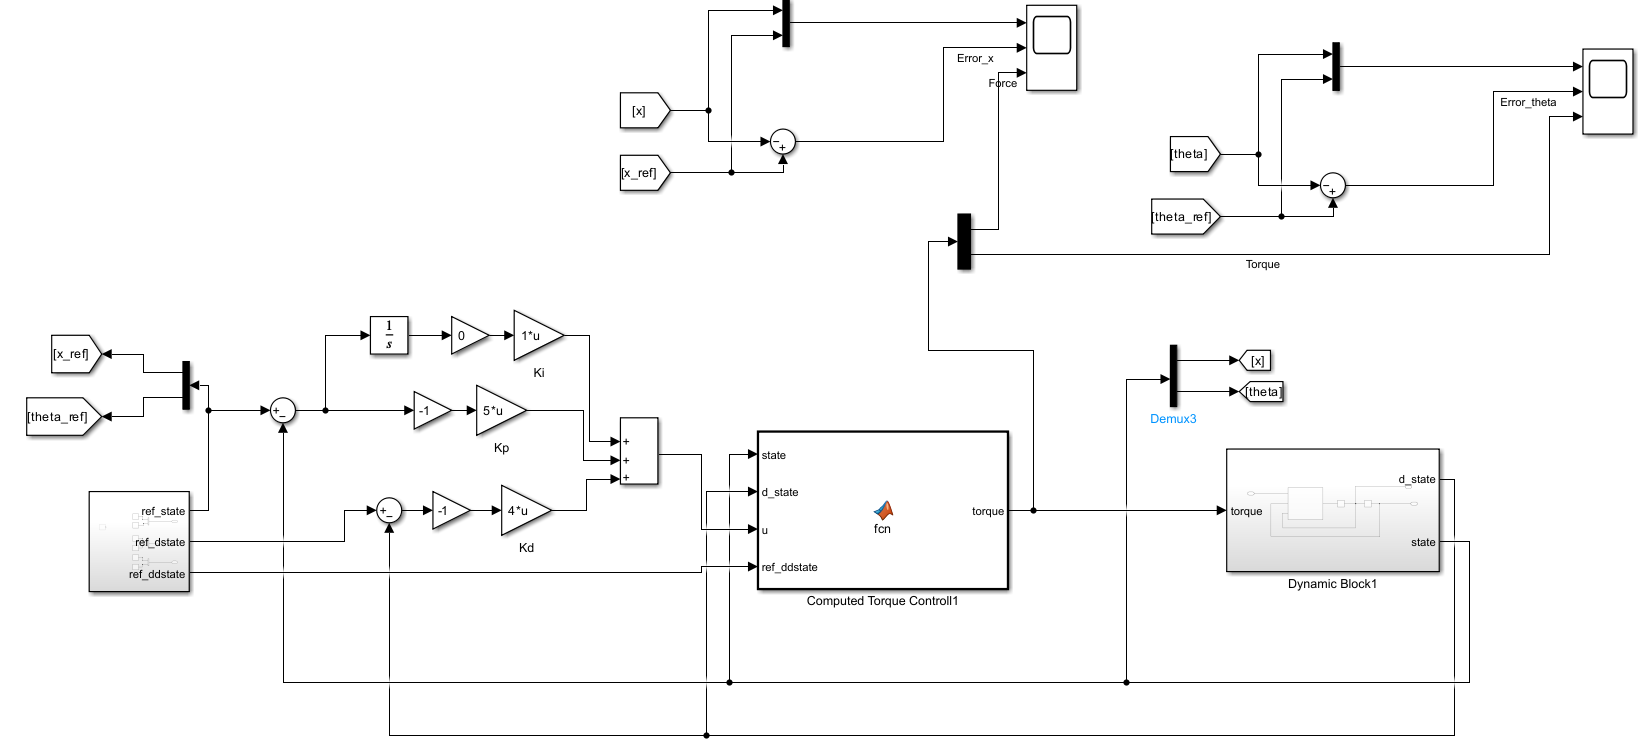
\includegraphics[width=1\textwidth]{pictures/ctc.png}
        \caption{Sơ đồ chung hệ thống điều khiển CTC}
    \end{figure}

    \section{Khối Dynamics}
    \begin{figure}[H]
        \centering
        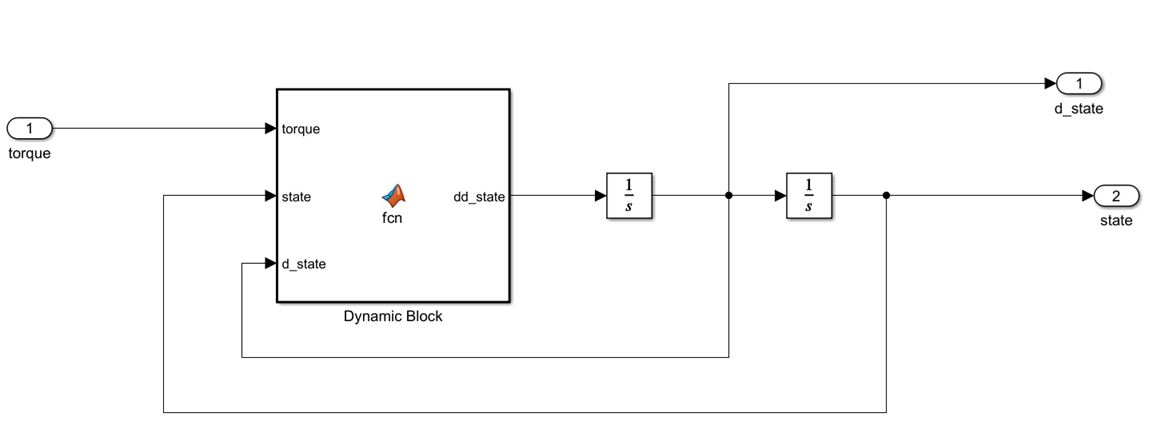
\includegraphics[width=1\textwidth]{pictures/dynamic_ctc.png}
    \end{figure}
    \begin{lstlisting}[caption={Code khối Dynamic Block}, label={lst:pz}]
        function dd_state = fcn(torque, state, d_state)
            % Define constant
            g = 9.81;
            r = 0.077;
            Mw = 0.3;
            Mp = 6;
            Iw = 0.0017;
            Ip = 0.29;
            l = 0.2;
            km = 0.0458;
            ke = 0.0458;
            R = 2.49;
        
        
            % Define variables
            x = state(1);
            theta = state(2);
            dx = d_state(1);
            dtheta = d_state(2);
    
            % Compute dynamic matrix
            M = ... 
            [Mp + 2*Mw + (2*Iw)/r^2, Mp*l*cos(theta);
                Mp*l*cos(theta),     Mp*l^2 + Ip];
            
            C =... 
            [0, -Mp*dtheta*l*sin(theta);
            0,                       0];
            
            V =... 
            [-Mp*dtheta^2*l*sin(theta);
                                    0];
            
            G = ...
            [                 0;
            -Mp*g*l*sin(theta)];
            
            B = [2/r; -2];
            
            % Compute acceleration
            dd_state = inv(M)*(torque - G - V); 
    \end{lstlisting}


    \section{Khối Computed-Torque Control + Input}
    \begin{figure}[H]
        \centering
        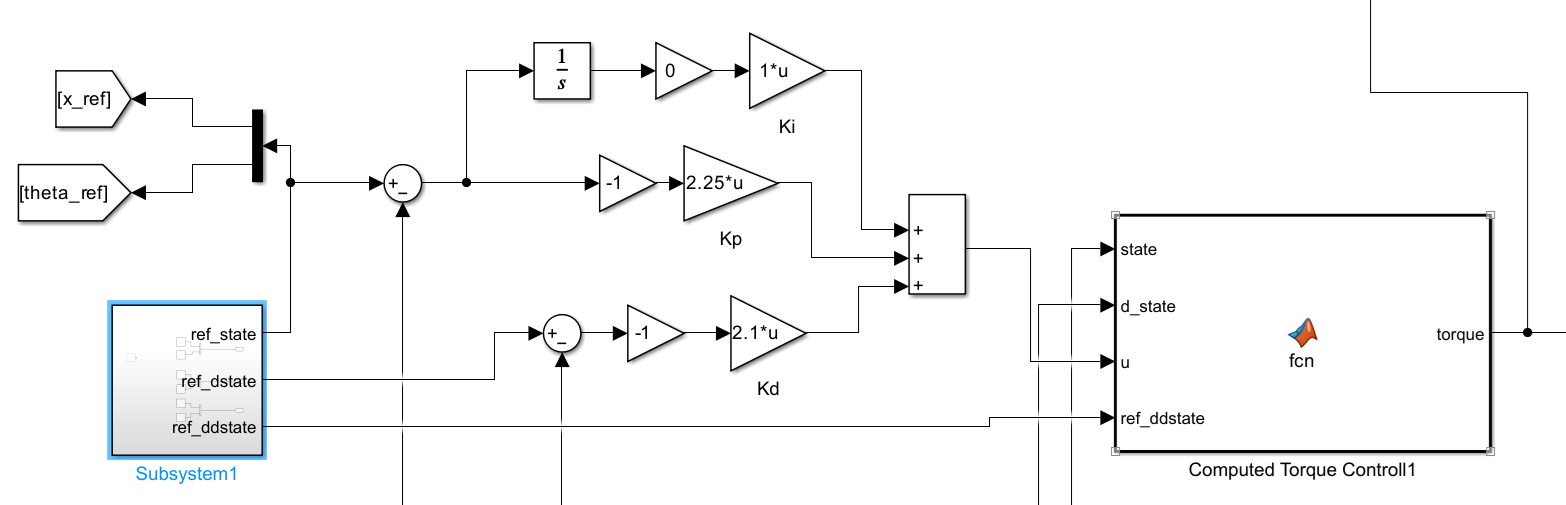
\includegraphics[width=1\textwidth]{pictures/ref_ctc.png}
    \end{figure}
    \begin{lstlisting}[caption={Code khối Computed-Torque Control}, label={lst:step}]
        function torque = fcn(state, d_state, u, ref_ddstate)
        % Define constant
        g = 9.81;
        r = 0.077;
        Mw = 0.3;
        Mp = 6;
        Iw = 0.0017;
        Ip = 0.29;
        l = 0.2;
        km = 0.0458;
        ke = 0.0458;
        R = 2.49;     
        
        % Define variables
        x = state(1);
        theta = state(2);
        dx = d_state(1);
        dtheta = d_state(2);
               
        M = ... 
        [Mp + 2*Mw + (2*Iw)/r^2, Mp*l*cos(theta);
               Mp*l*cos(theta),     Mp*l^2 + Ip];        
         
        C =... 
        [0, -Mp*dtheta*l*sin(theta);
        0,                       0];
         
         
        V =... 
        [-Mp*dtheta^2*l*sin(theta);
                                0];
         
         
        G = ...
        [                 0;
        -Mp*g*l*sin(theta)];
        
        
        
        B = [2/r; -2];
        B_dagger = pinv(B); 
        
        %tau is scalar
        tau = B_dagger * (M *(ref_ddstate - u) + V + G);

        
        torque = (M*(ref_ddstate - u) + V + G);       
    \end{lstlisting}



    
